\pagestyle{empty}
\frontmatter
%frontispiece
%\begin{figure*}[p]
%  	\centering
%  	\includegraphics[scale=0.2]{Durer/Albrecht_Dürer_The_Third_Knot.jpg}
%  	\caption{}
%  \end{figure*}
%\clearpage

\titleGM

\clearpage

%COPYRIGHT PAGE
\begin{vplace}[2]
\noindent
THE REVELATION OF JESUS CHRIST: \\READING IN LIGHT OF THE OLD TESTAMENT\\
\newline
Copyright \copyright 2022 by Caleb George\\
All rights reserved.\\
\newline
Printed in United States of America\\
\newline
Thank you for buying an authorized edition of this book and for complying with copyright laws by not reproducing, scanning, or distributing any part of it in any form without permission.
\newline
\newline
First Edition: March 2022
\newline
\newline
Scripture quotations marked CSB have been taken from the Christian Standard Bible®, Copyright © 2017 by Holman Bible Publishers. Used by permission. Christian Standard Bible® and CSB® are federally registered trademarks of Holman Bible Publishers.
\newline
\newline
Kephali Press
\newline
Athens, AL 35613
\end{vplace}

\clearpage
\clearpage

\dedication
\clearpage

\ClearShipoutPicture
\AddToShipoutPicture{%
   \checkoddpage
   \transparent{0.08}
   \ifoddpage
     \put(0,0){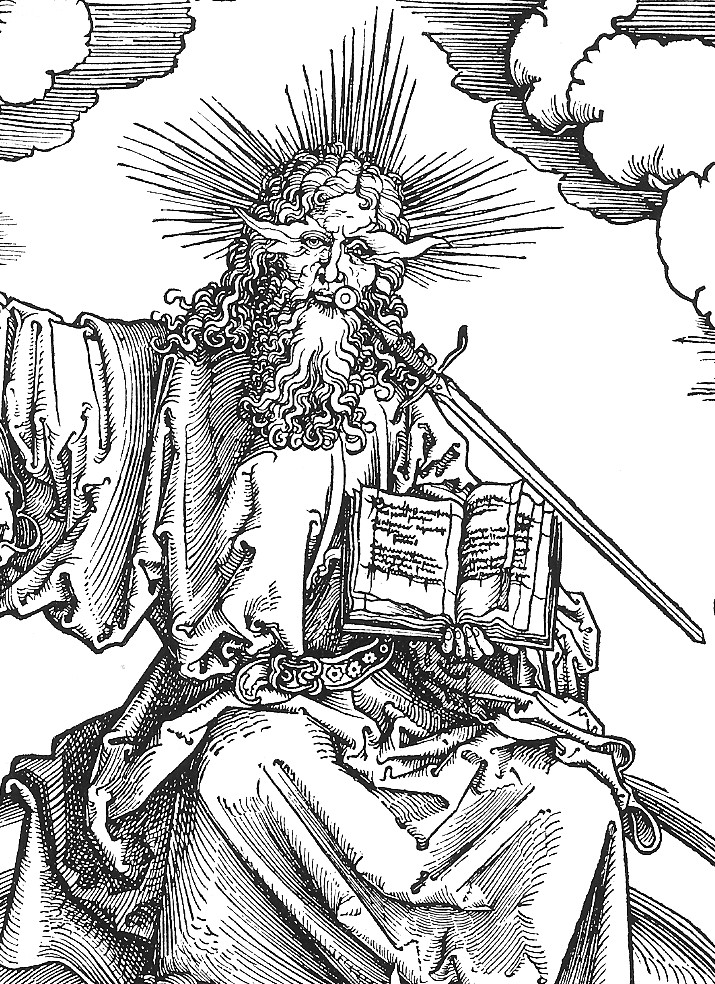
\includegraphics[width=\paperwidth,height=\paperheight]{Durer/Son_of_Man.jpg}}
   \else
     \put(0,0){\includegraphics[width=\paperwidth,height=\paperheight]{Durer/Dürer_Apocalypse_dragon.jpg}}
   \fi
}

\blankpage
\clearpage
\clearpage

\begin{KeepFromToc}
\tableofcontents
\end{KeepFromToc}
\clearpage
\listoffigures
\clearpage

%PREFACE
\chapter{Preface}
There are two things which many Christians have found to be most helpful in studying the book of Revelation: (1) Visualize the terrifying and wonderful things that Jesus showed John and (2) study the connections between the Apocalypse and the relevant Old Testament texts. This book is meant to aid in both endeavors, but especially the latter. \\

The Apocalypse is overflowing with citations and allusions to the Hebrew Bible. The Nestle-Aland 28\textsuperscript{th} edition of the Greek New Testament (\textsc{NA28}) includes more than 700 Old Testament cross references in the book of Revelation. Physically turning to all of these references in a hard copy of the Bible is not something the typical reader is inclined to do. Smartphone or tablet users may find it easier to click on a cross reference to view a text, but even this requires a break in concentration and may involve switching windows/pages. \\

The format presented in this book allows the reader to glance at the bottom of a page and immediately read relevant OT texts, enabling the user to rapidly form mental connections and deepen his or her understanding. Each reference text has been carefully curated to provide the greatest value possible to Bible students and I have tried to give as much context as page space constraints permit. I have deliberately avoided adding human commentary and interpretation to the footnotes; there are other books available which do a better job of it than I can. In most cases, it will be easy to see the relationship between the main text and the footnote text; some will require more careful study.\\

Apocalyptic literature is highly visual. The prophets Ezekiel, Daniel, Zechariah, etc. and the apostle John repeatedly use the phrase, ``I saw'' (Ez. \ibiblechvs{Ezekiel}(1:1); Dan. \ibiblechvs{Daniel}(4:5); Zech. \ibiblechvs{Zechariah}(1:8); Rev. 1:12). We do well to try to ``see'' the same things those men saw; we need to watch the movie before trying to explain it. I was blessed in the 11\textsuperscript{th} grade to have a Bible teacher, Steve Klein, who actually made us draw the visions in each chapter. This exercise, regardless of our artistic prowess, brought the text to life. Of course, a drawing of a vision is a two-dimensional, still-frame representation of a three-dimensional, dynamic experience. We must also remember that these visions were transmitted to us in words which the apocalyptic authors indicate were inadequate to truly describe what they saw - note the frequent use of ``like'' (Rev. 1:13, 15; 2:18; 4:3, 6, 7, etc.). But it is my hope that the woodcuts by Albrecht Dürer in his grand \textit{Apocalipsis cum Figuris}, first published in 1498, will stimulate your mind to look on with John at the glory, the wrath and the mercy of God and of the Lamb.\\
\fancybreak{* * *}
All Scripture in this book comes from the American Standard Version, unless otherwise noted. The \textsc{ASV} was chosen for three main reasons: it uses a strong formal equivalence approach to translation which is useful when comparing different texts, it is based on good manuscripts and, importantly, it is in the public domain. While some of the language is antiquated, this is an advantage with regard to pronouns. In 2:10 (\textsc{CSB}), when Jesus says, ``the devil is about\ldots\ to test you, and you will experience affliction for ten days,'' is he speaking to the church in Smyrna at large (singular ``you'') or is he speaking to individual Christians (plural ``you'')? The \textsc{ASV}'s use of \textit{ye} indicates the second person plural; in southern US vernacular, ``y'all will have tribulation''.\\

Some view the whole book of Revelation as ``a single poem'' and in at least one english version it has been rendered entirely in loose blank verse.\footnote{Willis Barnstone, \textit{The New Covenant, Vol. 1} (New York, NY: Riverhead Books, 2002), 380.} Most have taken a more conservative approach, presenting the book as a mixture of poetry and prose. While not a single word of the \textsc{ASV} text has been changed in this book, I have followed the example of the \textsc{NA28} text in formatting many sections as poetic verse, something the \textsc{ASV} did not do. On occasion I have also followed the \textsc{NA28} in punctuation and paragraph break decisions.\\

A note about the footnotes is in order. In an effort to provide as many relevant OT texts as possible, I found it necessary to abridge most of the verses quoted in the footnotes, eliminating words or phrases that did not bear directly on the main text. If an OT text was abridged in the middle, I have indicated so with ellipses (\ldots); if it was abridged at the beginning or end, I have not indicated that. The first letter of all footnote quotations is always capitalized regardless of the capitalization in the OT text and most footnotes end with a period (.), even if the OT verse does not have a period at that point.
\fancybreak{ * * *}
To God be the glory for providing such a rich variety of resources aimed at the study of His word. It is my hope that this book be as useful to you as the preparation of it has been to me. I would like to thank John Gibson for reviewing an early draft and providing feedback, my parents for their encouragement and especially my dear wife, Mabeliz, for her patience as I spent many hours colorizing the woodcuts pixel-by-pixel and writing countless tweaks to the \LaTeX{} script. This book is lovingly dedicated to her.\\
\\
Caleb George\\
Managua, Nicaragua\\
March 2022
\clearpage
\ClearShipoutPicture
\cleartorecto
\begin{vplace}
\begin{center}
\textit{
Woe is me! for I am undone; \\
because I am a man of unclean lips, \\
and I dwell in the midst of a people of unclean lips: \\
for mine eyes have seen the King, \\
Jehovah of hosts.} \\
-ISAIAH 6:5
\end{center}
\end{vplace}

